%\documentclass[]{article}
\documentclass[letterpaper, preprint, paper,11pt]{AAS}
\usepackage{amssymb}
\usepackage{amsmath}
\usepackage{graphicx}
\usepackage{amsthm}
\newtheorem{theorem}{Theorem}

% Title Page
\title{Entry Guidance for Propellant Optimal Powered Descent Ignition on Mars}


\PaperNumber{20-664}
\begin{document}
\author{Connor D. Noyes\thanks{Ph.D. Candidate, Department of Mechanical and Aerospace Engineering, University of California, Irvine, 92697} \ and Kenneth D. Mease\thanks{Professor Emeritus, Department of Mechanical and Aerospace Engineering, University of California, Irvine, 92697}}
\maketitle

%\begin{abstract}

%\end{abstract}


\section{Introduction}
Among the many considerable challenges involved in the Entry, Descent, and Landing (EDL) of a spacecraft on Mars, perhaps the greatest is the low density of the Martian atmosphere \cite{BraunMarsEDL, joel_dissertation}. At approximately one percent of the Earth's atmospheric density, current generation Mars entry vehicles are incapable of achieving sufficient deceleration to reach subsonic speeds before reaching the surface, necessitating the use of EDL technologies including supersonic parachutes and retropropulsion, both of which were utilized in safely landing MSL's Curiosity rover \cite{MSL_EDL}, and will also be utilized on the upcoming Mars 2020 mission \cite{M2020_EDL}. As the mass (or ballistic coefficient) of these vehicles grows, the problem is exacerbated until safe deployment conditions for current supersonic parachutes are not reachable at altitudes high enough to provide sufficient timeline margin for subsequent EDL events \cite{BraunMarsEDL}. In such missions, supersonic retropropulsion (SRP) may be relied upon to land larger, heavier vehicles relative to the current generation of landers without the use of a parachute, and as a result powered descent will play an even more significant role in the EDL process.  

%\textbf{It might be good to talk about the two phases here.}Figure~\ref{fig_phases} shows the two-phase EDL problem under consideration. 


The challenges during the entry phase from a guidance perspective include entry state dispersions due to delivery errors, atmospheric winds and density uncertainty, aerodynamic uncertainty, and imperfect onboard state estimation, each of which contribute to the size of the landing footprint. To date, MSL is the only Mars entry system to utilize hypersonic guidance to autonomously steer the spacecraft toward the target, which resulted in a landing footprint nearly an order of magnitude smaller than previous unguided ballistic entries \cite{BraunMarsEDL}. A common assumption pertaining to SRP-based EDL is the requirement of pinpoint accuracy, defined as a sub-100 meter landing ellipse \cite{GNC_Pinpoint}. Under such an assumption, dispersed entry trajectories result in increased propellant requirements, rather than contribute to the landing ellipse. As a result, rather than judge an entry guidance algorithm by its landing ellipse, the propellant cost or propellant mass fraction (PMF) of the powered descent trajectory may now be considered a primary metric.

A fundamental difference of retropropulsion-based EDL from parachute-based EDL architectures, even those that utilize a vertical powered descent phase with potential for a divert maneuver beforehand, lies in the set of desirable states at the termination of the entry phase. The terminal entry state is constrained by safe parachute deployment conditions defined by upper and lower limits on Mach number and dynamic pressure. The constraints are often translated into constraints on altitude and velocity using a model of the Martian atmosphere. In summary, when a chute is involved, the target set is the parachute deployment box coupled with small downrange and crossrange errors, combined with a well-aligned heading, and no restriction on flight path angle. Traditionally, the primary objective of bank angle modulation during entry is range control with lateral control as a secondary objective, and guidance approaches could treat the two problems as decoupled. During the mission design phase, the downrange distance is chosen to be compatible with the parachute deployment conditions and other mission parameters such as the entry flight path angle.

The target set in SRP-based EDL is in some sense much larger, but with more important coupling between the states. All six of the entry states contribute to the propellant cost; the optimal downrange distance and altitude at which to ignite depend on both the velocity magnitude and the flight path angle while aligning the heading is necessary to eliminate crossrange distance to the target. Altering the objective of entry guidance to shaping the trajectory for the benefit of the powered descent phase thus encourages a coupled approach. \textbf{This may not be as true with a low T/W ratio} 

%For example, MSL utilized a range control phase and a heading alignment phase. Once the heading is aligned, the bank angle command will remain zero until the termination of the entry phase. Thus, unless heading alignment is initiated at the right time for zero bank angle to lead to the best termination condition, blah blah.

The proposed entry guidance for SRP-based EDL begins with an analysis of the chosen powered descent guidance approach. The chosen algorithm will define a mapping from a given state to the propellant required to reach the target set. This mapping is computed over a set of interest and stored for use in the entry phase. Details of this computation are presented later. This mapping is utilized in two distinct ways. At points along a given entry trajectory, the propellant cost can be computed in order to determine the best ignition condition for that trajectory. If the trajectory does not intersect a portion of the feasible ignition set with sufficiently low propellant cost, the bank angle profile can be modified to improve the intersection using the mapping.  
%If the trajectory is poor, there may be not suitable ignition point, and the bank angle profile should be modified.

There exist many guidance solutions to the powered descent problem, with many focusing on propellant optimality. Such classes of algorithms include G-FOLD\cite{gfold,gfold_flighttests} and other convex optimization-based methods, polynomial-based approaches including the venerated Apollo lunar descent guidance \cite{apollo_lunar}, indirect optimal control methods \cite{PropellantOptimalAdaptiveTrigger}, and many others. In brief, there is no shortage of ways to tackle the problem of powered descent.

%There are several components of the entry guidance approach: mapping from SRP state to propellant cost, bank angle parametrization, and adaptive transition from entry to powered descent. 

Far less attention has been given to the role of entry guidance when followed directly by a powered descent phase, without an intermediate phase that makes use of a parachute or other decelerator. Reference~\cite{LuAdaptiveEDL} presents one approach to entry guidance in a chuteless EDL architecture. Although Ref.~\cite{LuAdaptiveEDL} correctly identifies the potential for integrating the entry phase with the subsequent powered descent phase as an opportunity to reduce propellant consumption, the vehicle's bank angle is still modulated to perform range control, utilizing a bank profile that is linear-in-energy with one parameter. Lateral logic to determine bank reversals is applied separately after solving for the bank angle magnitude. Reference~\cite{EDL_AllProp} investigated an alternative EDL scheme in which aerodynamic control during entry is foregone in favor of hypersonic retropropulsion, essentially eliminating the entry phase. 

A key component of our approach is an adaptive trigger for powered descent initiation.  In essence, the role of such a trigger is to ensure the minimum propellant ignition point is found along any entry trajectory. The theoretical developments behind one such trigger were introduced in Ref.~\cite{PropellantOptimalAdaptiveTrigger}, while Ref.~\cite{LuAdaptiveEDL} demonstrated its benefits over triggering at a fixed state variable such as downrange, velocity, or energy.
One potential weakness of this version of the trigger is that it assumes a propellant optimal powered descent guidance. In theory, future Mars missions, especially those transporting humans, may very well consider a guidance algorithm with a different objective, such as prioritizing safety or even passenger comfort, as the bang-bang nature of propellant optimal powered descent solutions may not be suitable despite the importance of limiting propellant consumption. 

%That trigger is only called on current state. 
Despite presenting an approach in which a prediction of the terminal entry state is available and being used to modulate the vehicle's bank angle, in Ref.~\cite{LuAdaptiveEDL} only the current vehicle state is checked for triggering the powered descent initiation. Our approach to the triggering mechanism differs in that we utilize the predicted trajectory. This allows us to query the mapping from the powered descent guidance algorithm at points along the predicted trajectory to generate propellant consumption predictions.  The benefit of doing so is two-fold. Firstly, the propellant optimal ignition point along an entry trajectory can be determined for \textit{any} subsequent powered descent guidance, even one that is itself not propellant optimal. Secondly, by making explicit use of these predictions in the entry guidance algorithm, the two phases become linked by more than just the adaptive trigger, and superior propellant performance can be achieved. 

%Despite attemps to coordinate EG+PD...
%Although Ref.~\cite{LuAdaptiveEDL} correctly identifies the potential for integrating the entry phase with the subsequent powered descent phase as an opportunity to reduce propellant consumption, the vehicle's bank angle is still modulated to perform range control, utilizing a bank profile that is linear in energy with one parameter. Lateral logic to determine bank reversals is applied separately after solving for the bank angle magnitude. In our approach, lateral and longitudinal motions are not decoupled, and thus the minimum number of parameters we consider in our parametrization is two. %This complicates optimization of these parameters, but the tradeoff is worth making if fuel expenditure is prioritized over computational burden. Even then, the approach can reduce time by storing some solutions computed offline. 

%Additionally, as mentioned above, our proposed entry guidance approach utilizes the powered descent guidance to be employed in the subsequent phase, in order to generate predicted propellant costs along a predicted trajectory. In this approach, the bank angle is actively modulated to reduce predicted propellant consumption rather than achieve a range objective, thereby allowing the entry guidance algorithm to suitably shape the trajectory in preparation for powered descent. It is this coordinated effort that allows the proposed entry guidance to produce superior results over traditional entry guidance methods. 

%We note that Reference Fully-Propulsive Mars Atmos Strategies for High-Mass Payload Missions looked at chuteless architectures but did not utilize lifting for control, and instead employed HYPERsonic retropulsion.
\subsection{Problem Statement, Definitions, Coordinate Frames}
The problem under investigation considers a two-phase EDL sequence consisting of an entry phase and a powered descent phase. An approach phase is generally not modeled as part of the EDL sequence, and the dispersions arising from this phase are modeled as delivery errors. In the entry phase, the vehicle is guided via bank angle modulation and the vehicle state is described in spherical coordinates. In the descent phase, the vehicle is guided via supersonic retropropulsion with the equations of motion given in Cartesian coordinates.  The reason for the choice of two different coordinate systems is to be consistent with the literature on each respective topic.

\begin{figure}[h!]
	\centering
	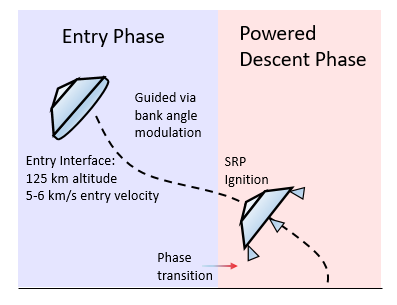
\includegraphics[width=0.7\textwidth]{EDLPhaseDiagram} 
	\caption{Schematic of the EDL phases}
	\label{fig_phases}
\end{figure}

The planet-relative equations of motion for a vehicle, modeled as a point mass, in unpowered flight through an atmosphere, in spherical coordinates, are
\begin{align}
\dot{R} &= V\sin\gamma \label{eq_entry_start}\\
\dot{\theta} &= \frac{V}{R}\frac{\cos\gamma\cos\psi}{\cos\phi}\\
\dot{\phi} &= \frac{V}{R}\cos\gamma\sin\psi \\
\dot{V} &= -D - G\sin\gamma \\
\dot{\gamma} &= \frac{L}{V}\cos\sigma + (\frac{V}{R}-\frac{G}{V})\cos\gamma + C_{\gamma}\\
\dot{\psi} &= -\frac{L}{V}\frac{\sin\sigma}{\cos\gamma} - \frac{V}{R}\cos^2\gamma\cos\psi\tan\phi + C_{\psi}\label{eq_entry_end}
\end{align}
where $R$ is magnitude of the vehicle's radial distance from the center of the planet, $\theta$ and $\phi$ are the longitude and latitude of the vehicle, $V$ is the magnitude of the vehicle's velocity vector,  $G=\mu/R^2$ is the magnitude of the gravitational acceleration, $\gamma$ is the flight path angle, $\psi$ defines the vehicle's heading, measured counterclockwise from East, and $\sigma$ is the bank angle of the vehicle. The Coriolis terms $C_{\gamma},\,C_{\psi}$ are equal to
\begin{align}
C_{\gamma} &= 2\omega\cos\psi\cos\phi \\
C_{\psi} &= 2\omega(\tan\gamma\sin\psi\cos\phi-\sin\phi)
\end{align}
where $\omega$ is the rotation rate of Mars. Equations~\ref{eq_entry_start}-\ref{eq_entry_end} will be compactly referred to as $\dot{x} = f(x,\sigma)$ and their solution at time $t$ from a state $x_0$ evolving under a bank angle profile $\sigma[0,t]$ is given by the transition map $x(t) = T[x_0;\sigma[0,t]]$.

The equations of motion for a point mass vehicle in powered flight are
\begin{align}
&\dot{r} = v \label{eq_eom_srp} \\
&\dot{v} = \frac{T}{m} + g(r) \\
&\dot{m} = -\frac{||T||}{I_{sp}G_0} \label{eq_eom_srp_end}
\end{align}
where $r\in\mathbb{R}^3$ is the position vector of the vehicle, $v\in\mathbb{R}^3$ is the velocity vector of the vehicle, $m$ is its mass, $T\in\mathbb{R}^3$ is the thrust vector of the vehicle, $g\in\mathbb{R}^3$ is the gravitational acceleration vector, $I_{sp}$ is the specific impulse of the rocket engine, assumed to be constant, and $G_0$ is the gravitational acceleration magnitude at the surface of the Earth. The full state vector in $\mathbb{R}^7$ comprises the position, velocity, and mass. 

The powered descent problem considered herein is to determine the optimal thrust magnitude and direction, as well the optimal time of flight, subject to the equations of motion and constraints on the available thrust.  The initial powered descent state is assumed to be fixed and the target position and velocity are taken to be $[0,\, 0,\, z_{target}]$,  $[0,\, 0,\, \dot{z}_{target}]$ respectively, where $z_{target}$ and $\dot{z}_{target}$ are the desired altitude and vertical velocity at the end of the descent phase. The optimal control problem is posed as
\begin{align}
\max \;m(t_f) \label{eq_srp_ocp}\\
&r(t_0) = r_0 \\
&v(t_0) = v_0 \\
&m(t_0) = m_0\\
&r(t_f) = [0,\, 0,\, z_{target}] \\
&v(t_f) = [0,\, 0,\, \dot{z}_{target}] \\
&T_{\min} \le ||T(t)|| \le T_{\max}
\end{align}
together with the dynamics Eq.~\ref{eq_eom_srp}-\ref{eq_eom_srp_end}. Formulated as such, the optimal control problem can be viewed as a function $\mathrm{OCP}(\cdot)$ that maps an initial condition, or ignition state, to a propellant cost. The set of all initial state vectors for which the optimal control problem is feasible and the propellant required by the solution less than some prescribed maximum $ M $ is $X_{M} = \left\{x\,|\, \mathrm{OCP}(x) \le M \right\}$.

Given an entry state and target position, the corresponding descent state is determined by assuming the current heading $\psi$ defines the downrange distance. The downrange and crossrange distances to the target are computed via spherical trigonometry \cite{joel_dissertation}
\begin{align}
d &= \cos^{-1}\left(\sin\phi\sin\phi_{target} +\cos\phi\cos\phi_{target}\cos(\theta_{target}-\theta)        \right) \\
\Psi &= \pi/2 - \mathrm{sign}(\theta_{target}-\theta) \cos^{-1}\left(\frac{\sin\phi_{target}-\sin\phi\cos d}{\cos\phi\sin d}  \right) \\
c &= \sin^{-1}\left(\sin d\,\sin(\psi-\Psi))\right) \\
\end{align}
\begin{align}
DR &= r_p\cos^{-1}\left(\frac{\cos d}{\cos c}\right)\\
CR &= r_pc
\end{align}
where $r_p$ is the planet radius. The altitude above the target is computed simply by subtracting the target altitude $h_T$ from the current altitude $h = R-r_p$ and the full SRP state vector is $[DR,\, |CR|,\, h-h_T,\, -V\cos\gamma,\, 0,\, V\sin\gamma,\, m_0]$. Because the downrange direction is defined by the current heading angle, the crossrange velocity is always zero, allowing the use of 5-D interpolation rather than 6-D. The absolute value of the crossrange distance is used because this gives a denser table of tabulated solutions by exploiting symmetry resulting from the zero crossrange velocity. 

An alternative mapping from entry states to powered descent states is to convert the entry state and target to Cartesian coordinates and subtract them. Although this is a feasible option, it is not preferable because it would result that every entry state maps to a unique SRP state. This is undesirable because it requires a larger table of solutions encompassing all the possible Cartesian states. Instead, by using a downrange-crossrange coordinate system based on the current heading, an infinite number of entry states map to the same SRP state as a result of this surjective transformation. Intuitively, this reflects the rotational symmetry of the problem, stemming from the fact that states $ x $ and $ y $ have identical dynamics. More formally, for the powered descent problem as posed, any initial state $[ x,\, y,\, z,\, \dot{x},\, \dot{y},\, \dot{z},\, m]$ such that $(z, \dot{z}, m)$ are fixed and 
\begin{align}
x^2 &+ y^2 = p^2 \\
\dot{x}^2 &+ \dot{y}^2 = v^2 \\
\psi &= \tan^{-1}(y/x) \\
\dot{x} &= -v\cos\psi \\
\dot{y} &= -v\sin\psi \\
\end{align}
lies along an iso-propellant contour. This essentially says that as long as the velocity vector is in the direction of the target, the propellant cost is dictated by the constants involved.
\begin{figure}[h!]
	\centering
	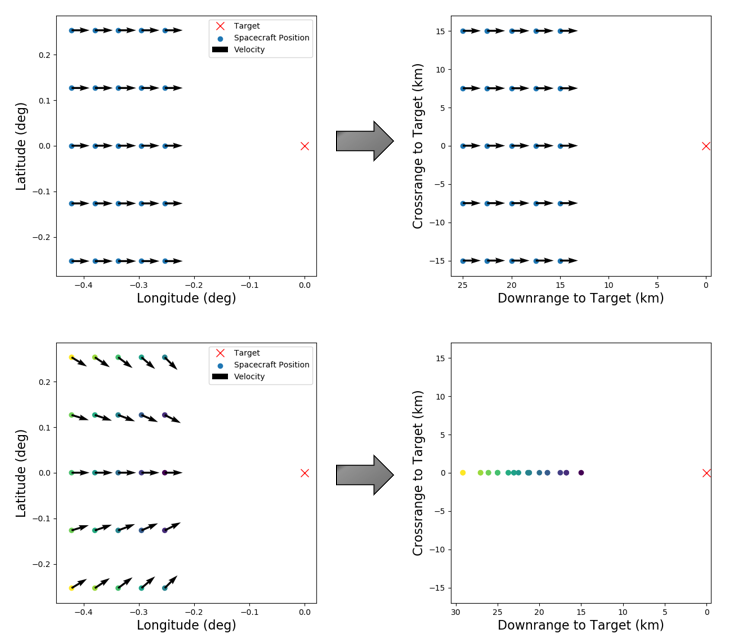
\includegraphics[width=1\textwidth]{EntryToSRP} 
	\caption{When the velocity is not aligned, each position maps to a different downrange-crossrange pair. In contrast, when the velocity vector is aligned with the target, all the states are mapped to zero crossrange.}
	\label{fig_entry_to_srp}
\end{figure}

%TODO: Show contours with and without heading alignment, also show how with HA they all map to the same crossrange
%TODO: Define sets of interest? Adapt definitions from Joel's dissertation

%TODO: Define the actual "optimal control problem" for the entry guidance: find the optimal state that is reachable from the current state and the bank angle profile that will deliver the vehicle to that state 

%Because the vehicle's altitude is often used as a proxy for remaining time to the ground, a minimum altitude is used to define the boundary of the reachable set. Actually, use the feasible set instead. 

The reachable state from a state $x$ is an entire tube of trajectories satisfying the equations of motion under admissible control trajectories $R(x)=\left\{x_f \,| \,\exists\, t_f \ge 0 \land\, \sigma[0,t_f] \,\mathrm{with}\, x_f = T[x; \sigma[0,t_f]]  \right\}$, but the portion of the reachable set that is of interest is its intersection with the feasible set, or $R \cap X_M$.

Unlike the powered descent optimal control problem, which may be solved on the ground to full optimality under no such parametrization, this problem is intended to be solved onboard and so motivates a low-order parametrization. The P-parametrized bank angle profile is a function of a finite set of parameters $P = \left\{p_1, p_2, ... \right\}$ that defines the bank angle for each state, $\sigma(x(t)) = \Sigma(x(t); P)$.

The P-parametrized reachable set is $R_P(x) =\left\{x_f \,| \,\exists\, t_f \ge 0 \land\, Q \,\mathrm{with}\, x_f = T[x; \Sigma(x; Q)[0,t_f]]]  \right\} $. The relative size of $R_P \subset R$ is not the most important consideration in choosing a parametrization. Instead, it is desirable that $R_P$ retains the the propellant optimal point (and neighboring region) while also not being too restricted in its size. More formally, in addition to considering the effects of a parametrization on some measure of $R_P\cap R$, one may also consider the optimality gap, 
\begin{align}
\delta m = \min_{x\in (R\cap X_M)} \mathrm{OCP}(x)\; - \min_{x\in (R_P\cap X_M)} \mathrm{OCP}(x) \ge 0
\end{align}
This may be difficult to compute in practice, in particular the lower bound set by the true optimum $\min_{x\in (R\cap X_M)} \mathrm{OCP}(x)$. Nevertheless, any two parametrizations can be compared via a similar computation. 
Figure~\ref{fig_sets} depicts the relationship between the sets $X_M,\,R,\,\mathrm{and}\,R_P$ as well as a possible situation to emphasize the previous point, wherein parametrization A encompasses less of $R$ yet has a smaller optimality gap than parametrization B. 
%TODO: Explain further 

\begin{figure}[h!]
	\centering
	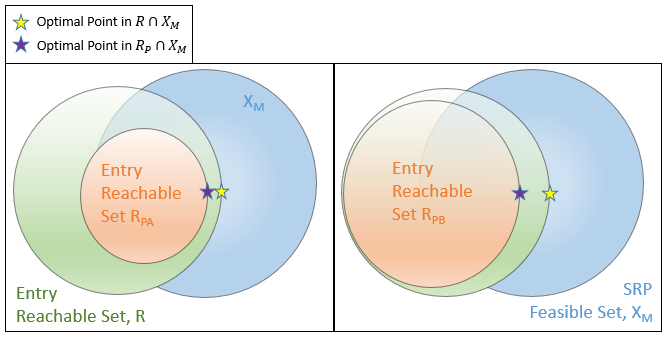
\includegraphics[width=0.8\textwidth]{SetDefinitions} 
	\caption{Consider two different parametrizations of the control, $ P_A $ and $ P_B $. Despite $ R_{P_B} $ being a larger set encompassing more of the true reachable set $R$, the intersection $R_{P_A}\cap X_M$ is ``larger" than $R_{P_B}\cap X_M$ and more importantly $ R_{P_A} $ encompasses a key subset of $ R $ – the region near the optimum. The difference between the two different optima is the sub-optimality gap imposed by the chosen parametrization.}
	\label{fig_sets}
\end{figure}

 

%Viewing the trajectory as a function of the control input u, determine the optimal u* and ignition velocity v* such that $x(v*; u*)\in X_M$ 
%$\min_u^* OCP(entry2srp(x(u*)))$


\section{Proposed Entry Guidance}

%Components of entry guidance: 
%Bank angle parametrization
%SRP guidance -> N-D table of propellant costs -> Required to determine both hand off state and params to get there 
%Onboard determination of ``handoff" i.e. transition from Entry phase to SRP phase 

The objective is deliver the vehicle to the minimum propellant point in the feasible set $X_M$ that is reachable under the chosen bank angle parametrization from the current state. This is in contrast to prescribing ad hoc rules for the terminal entry set to reduce propellant consumption, such as minimizing velocity at a certain downrange distance to the target. 
%Seeking the optimal point requires that the terminal entry state be free of such constraints, i.e., it cannot be required to lie on a manifold defined by a fixed velocity or distance from the target. 

This objective is accomplished by the guidance algorithm using an inner/outer loop structure. In the inner loop, the propellant map is used to determine the optimal ignition point along each predicted trajectory. In the outer loop, the bank angle profile is optimized to find the optimal ignition state that is reachable from the current vehicle state, subject to the chosen parametrization of the bank angle profile. Thus, the three key components of the approach are the powered descent propellant map, the bank angle parametrization, and the onboard determination of the handoff condition at which the entry phase ends and powered descent begins.

%The Powered descent guidance defines a mapping from ignition states to propellant required. This mapping implicitly defines the SRP-feasible set. Although at no point do we explicitly compute this set, 

%At each cycle, the entry guidance algorithm seeks to determine the optimal ignition state as well as a bank angle profile that will guide the vehicle to that state.
 

%Sketch of algorithm: 
%(2-D) Optimization of objective function over bank profile parameters
%
%Objective function(parameters; current state)
%Integrate current state bank profile forward to target downrange distance
%Filter the predicted trajectory for constraints
%1-D search over remaining trajectory points to find minimum
%
%SRP guidance -> size of feasible set
%Bank parametrization + vehicle characteristics -> reachable set
\begin{figure}[h!]
	\centering
	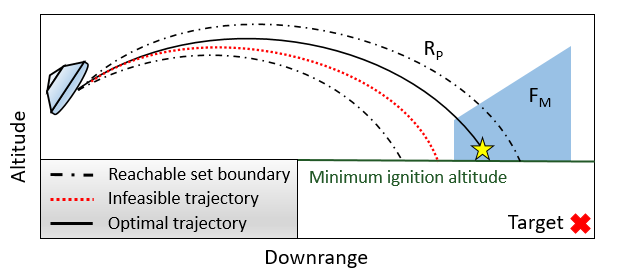
\includegraphics[width=0.8\textwidth]{Optimization} 
	\caption{The guidance algorithm seeks both the propellant-optimal ignition point (indicated by stars on the plot) and the trajectory whose optimal ignition point is best (indicated by the solid black line).}
	\label{fig_optimization}
\end{figure}

%At the core of the proposed entry phase guidance approach is an extension of the trajectory prediction to include the following powered descent phase. This allows one to alter the entry guidance objective from range control to propellant minimization. After applying several constraints to filter down the set of potential ignition states, the powered descent guidance is used to generate predictions of the propellant required from different states. The lowest among them is selected as the planned handoff condition from entry to powered descent. Further details on these constraints are given later.

%Notice that although propellant minimization is the entry guidance objective, any powered descent guidance algorithm with pinpoint landing capability may be used in the powered descent phase so long as an estimate of the propellant required is given by the algorithm, and this estimate is continuous with respect to the initial state. Thus, although in the examples of this work we have coordinated the powered descent phase to also be propellant-optimal in nature by solving the associated OCP, there exist many alternatives such as energy-optimal guidance or non-optimization based approaches such as polynomial guidance. 

%We further assume that the chosen powered descent method incorporates any necessary problem constraints, because the entry guidance algorithm does not make use of the predicted powered descent trajectory, nor does it check for satisfaction of constraints, but instead utilizes only the propellant cost associated with the powered descent trajectory. 

\subsection{Bank Angle Parametrization}

The commanded bank angle profile considered here is a constant bank angle magnitude $\sigma_c$ with one bank reversal at a velocity $v_r$
\begin{equation}
\sigma(v; \sigma_c, \,v_r) = \left\{
\begin{array}{ll}
\sigma_c & v\geq v_r \\
-\sigma_c & v < v_r
\end{array} 
\right.
\end{equation}
which is fed to a first order filter to approximate the nature of a reaction control system tracking the commands. Because the profile includes a reversal, it offers a means to control lateral motion. 

In our implementation, it is always assumed there is at most one reversal left, but the parametrization remains the same after each reversal. This allows for as many reversals as there are optimization updates, but in practice it is rare to see more than two reversals. With $v_r$ as an optimization variable with a sufficiently low bound, there exists the possibility to have one or no reversal planned at each update.  

\subsection{Powered Descent Propellant Mapping}
By repeatedly solving the optimal control problem, Eq.~\ref{eq_srp_ocp} for a set of initial conditions, a pointwise approximation of the true 5-D pinpoint landing feasible set $X_M$ is computed via sampling. A consequence of the dimensionality of the input space is a requirement to compute a large number of solutions - it takes 16,807 solutions to span each dimension with only 7 points. From these sampled solutions we construct a model of $X_M$. 

This mapping may be modeled in a variety of ways. Neural networks and other machine learning approaches were considered for their universal function approximation property. However, upon examination of the shape of the 5-D space together with numerical validation (a concept from machine learning) using additional OCP solutions, piecewise-linear 5-D interpolation was chosen to represent the propellant mapping.

The set of initial conditions over which to solve OCP is computed by Latin Hypercube Sampling. Constraints are applied to eliminate easily identified infeasible scenarios such as starting very near to the ground with significant downward velocity. In practice, the optimal region is generally not known in advance. 
\textbf{WIP}
%TODO: Iterative scheme
 

\subsection{Trajectory Prediction and Powered Descent Ignition}
Once the bank angle parametrization is specified, the estimated entry state is integrated numerically to generate a prediction of the remaining unpowered entry flight. The numerical integration of the entry state is carried out using downrange distance to the target as the independent variable. Using range to go as the independent variable allows the terminal integration condition to be zero, independent of the problem specifics, with very little wasted integration time since the optimal ignition state is generally close to the target. 

This has several advantages over common alternatives. First, although energy or velocity could be used, a sufficiently low choice of the terminal value must be made, but any time spent integrating below the reachable set of the vehicle is wasted, and the choice is problem/vehicle specific. Altitude would also be a natural choice since the minimum ignition altitude would serve as the terminal integration condition, but like energy and velocity this is problem-dependent, and additionally altitude is not a strictly monotonic variable in the case of lofting trajectories.

\begin{figure}[h!]
	\centering
	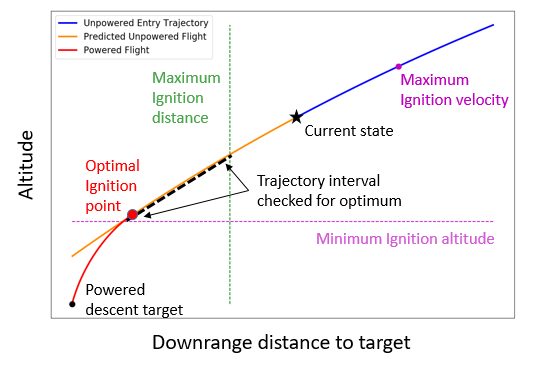
\includegraphics[width=0.9\textwidth]{H_Vs_S} 
	\caption{Only the interval of the predicted entry trajectory satisfying constraints on velocity, altitude, and distance to the target are searched for the propellant-optimal ignition state.}
	\label{fig_ignition}
\end{figure}

Once the prediction is generated, several constraints are applied to determine the interval of the trajectory that should be checked for the propellant optimal transition to powered descent. These constraints greatly reduce the number of calls to the descent guidance propellant mapping required to find the optimum. These constraints include an upper bound on velocity corresponding to the maximum achievable deceleration with the available propellant, a minimum ignition altitude required for safe powered descent and subsequent EDL operations, and a maximum distance to the target, again related to the available propellant. Figure~\ref{fig_ignition} depicts this process including a portion of the trajectory already flown, the entry flight prediction, constraints, pinpoint landing target, and predicted optimal ignition point. Once the constraints have been applied, 1-D optimization is applied to the remaining trajectory interval, indicated by the dash black line, by viewing the fixed trajectory as a function of some independent variable. Our implementation uses velocity as the independent variable over which to search, but time or distance are also possibilities. 1-D optimization is used to very quickly locate the optimum, rather than brute force the solution by checking all of the remaining points. 

\begin{figure}[h!]
		\centering
		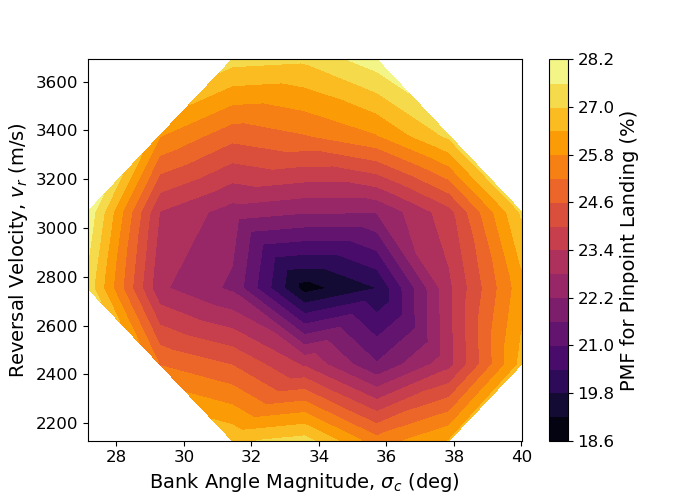
\includegraphics[width=0.9\textwidth]{ConstantBankObjective} 
		\caption{Contours of the propellant cost of pinpoint landing using a constant bank angle with one reversal, initial T/W = 4.}
\end{figure}
\begin{figure}[h!]
		\centering
		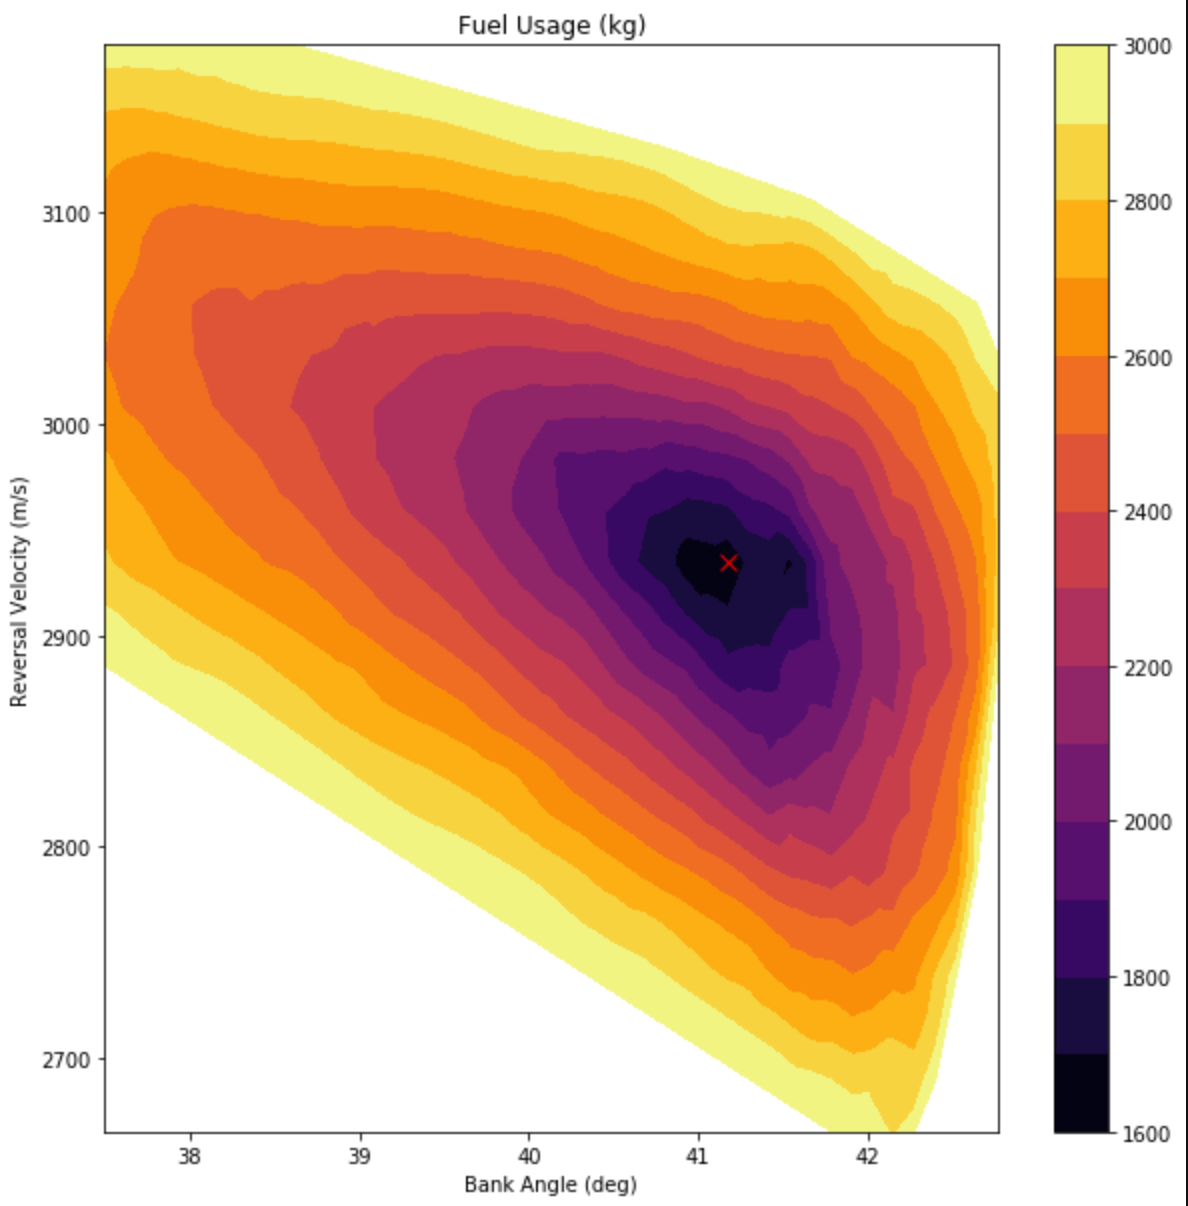
\includegraphics[width=0.9\textwidth]{Profile1_Objective} 
		\caption{Contours of the objective function using a constant bank angle with one reversal, initial T/W = 16.}
\end{figure}
%\subsection{Optimization}
%
%\subsubsection{Objective Function}
%The entry guidance requires that the chosen powered descent guidance approach admits continuous propellant requirements for continuous ignition states to a fixed target. Atmospheric entry dynamics are smooth for smooth bank angle inputs and we thus expect that even when optimizing the ignition condition along a trajectory rather than use a fixed state variable such as velocity or energy, the objective function should be well-behaved and amenable to optimization. One key question is whether several isolated minima exist, or only a single global optimum. 
%
%Evaluating the objective function for a range of parameters for the bank profile as was done to generate Figure~\ref{fig_contour} indicates the objective function is bowl shaped with very steep gradients away from the optimum. From this, and repeated optimizations at various possible points, there is always a clear optimum.
%
%The shape of the objective function indicates that gradient-based methods will be effective in determining the optimal profile parameters, however, determining the gradient of the objective function with respect to the switching velocity is generally difficult. As a result, derivative-free methods are preferred for this application. Powell's conjugate direction method is used in all of the examples herein. It is effective because once an appropriate search direction is identified, the problem is reduced to a bounded one-dimensional search. 
%
%Contours of the optimal parameters corresponding to the solutions in Figure~\ref{fig_contour} are given in Figures~\ref{fig_bank} and \ref{fig_rev}. Immediately striking is the optimal bank angle's clear independence from azimuth errors; instead, it is dictated entirely by the flight path angle. 
%\begin{figure}[h!]
%	\centering
%	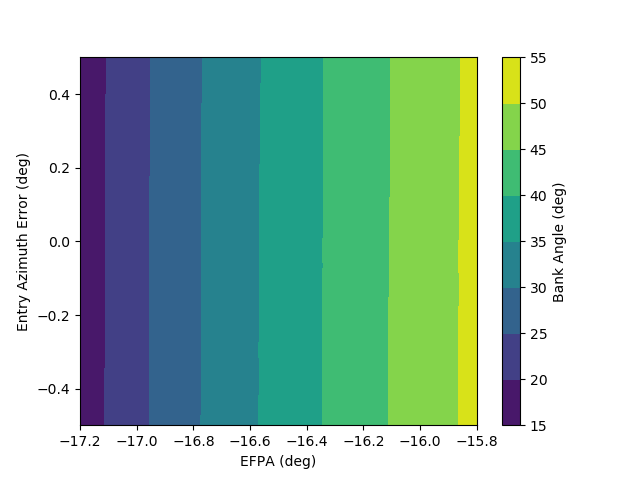
\includegraphics[width=1\textwidth]{optimal_bank} 
%	\caption{Optimal bank angle for different entry flight path angles and heading angles.}
%	\label{fig_bank}
%\end{figure}
%
%\begin{figure}[h!]
%	\centering
%	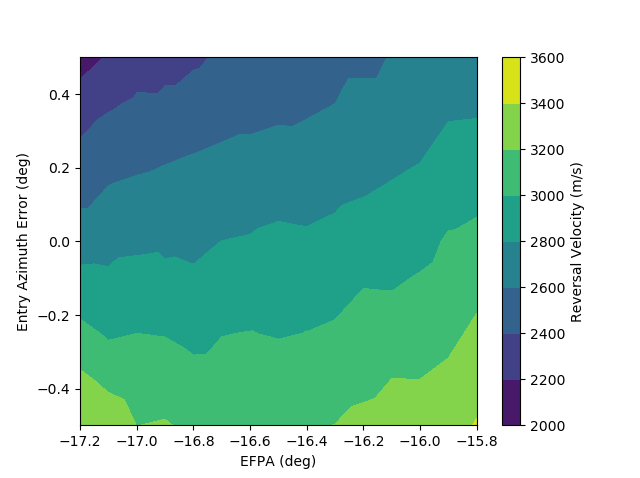
\includegraphics[width=1\textwidth]{optimal_reversal} 
%	\caption{Optimal reversal velocity for different entry flight path angles and heading angles.}
%	\label{fig_rev}
%\end{figure}
%
%
%\pagebreak
\section{Results/Performance}
%TODO: Like the range error breakdown for different disturbances, show the propellant increases caused by different disturbances - i.e. sensitivity study ish?}

%TODO: Stability of predicted ignition conditions and propellant use over time. These variables form a path

%TODO: Seemingly very little variation in terminal entry state for different EFPA/AZI. But a standard feedback controller couldn't accomplish that 

%TODO: Do all of the trajectories feature lofting? It's likely a feature related to altitude maximization 

%TODO: Monte Carlo Filtering if monte carlo results 

\textbf{Work in progress}

The performance of the algorithm is first investigated in a series of one-dimensional sensitivities to parametric uncertainties, including lift and drag coefficients, and two forms of density uncertainty. Entry state dispersions are also examined. 

\begin{table}[h!]
	\centering
	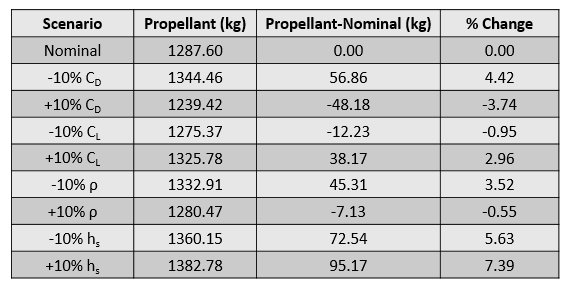
\includegraphics[width=0.75\textwidth]{ParametricSensitivityTable} 
	\caption{A summary of propellant costs for a series of $\pm10\%$ uncertainties compared to a nominal scenario with no uncertainty.}
	\label{table_parametric}
\end{table}

\begin{table}[h!]
	\centering
	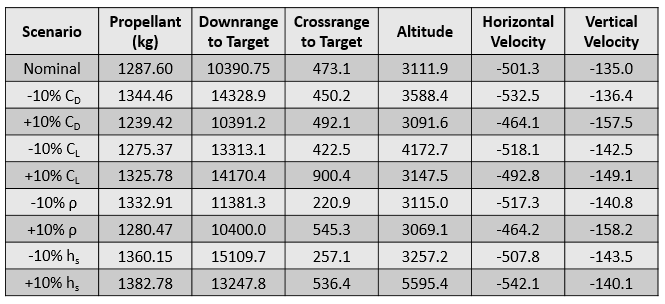
\includegraphics[width=0.75\textwidth]{ParametricSensitivityIgnitionTable} 
	\caption{A summary of the propellant-optimal ignition states for a series of $\pm10\%$ uncertainties. Optimal trajectories generally feature low crossrange, and altitudes close to the minimum altitude constraint.}
	\label{table_parametric_ignition}
\end{table}

%Due to their similar effect on the vehicle's L/D ratio, the perturbations pairs  $ +C_D $, $ -C_L $ and $ -C_D $, $ +C_L $ result in essentially the same update to the bank angle magnitude. The lift dispersed cases essentially fly identical altitude-velocity profiles but have slightly different reversal velocities due to the impact of lift on lateral motion. 

%Due to its reliance on predictions, the algorithm is susceptible to model uncertainty. Reference~\cite{predictor_corrector_analysis} examined the performance of predictive algorithms under such circumstances and found, like Ref.~\cite{lu2014entry}, that model adaptation during flight is essential to good performance in the presence of such parametric uncertainty. 
Table~\ref{table_parametric} summarizes the propellant usages and compares them to the nominal scenario, while Table~\ref{table_parametric_ignition} gives the corresponding propellant optimal ignition states. Several trends are noticeable. The terminal altitude is almost always very close to the minimum altitude constraint. This allows the vehicle to decelerate as much as possible, reducing the velocity that must be nulled by SRP. Scenarios in which the optimal ignition occurs higher indicate some other constraint is active, such as overshooting the optimal downrange distance at which to ignite. Additionally, all of the trajectories feature lofting nearly the end of the entry phase, again allowing for additional deceleration prior to ignition. 

Although there is no separate guidance logic for heading alignment, it is clear from the small crossrange values in Table~\ref{table_parametric_ignition} that by using the table of SRP solutions, the vehicle does align its heading prior to ignition. Not only that, but it times the reversal such that heading is aligned at the right time but without sacrificing range performance. 
%Although the solutions are generally aligned, we can see another strength of the method is that there may be times when accepting some crossrange error in order to improve other states is a worthwhile tradeoff, and this determination is made on a numerical basis.

% For a fixed ground target, a wide range of entry flight path angles (EFPAs) and entry heading errors can be accommodated by the entry guidance algorithm. Figure~\ref{fig_sweep} is an example that demonstrates the propellant cost is approximately invariant with respect to entry azimuth errors and varies weakly with EFPA, about 200 kg of propellant over $1.4^\circ$ of variation in EFPA. The range of acceptable EFPAs is often set by considerations such as g-load limits, or aerothermal constraints, and these results indicate such constraints can be imposed at little-to-no cost to propellant. 
%
%It is expected that a guidance algorithm that provides range control during entry to the same downrange distance over such a range of EFPAs will fly very different entry trajectories with a much greater variance in the propellant cost to decelerate the vehicle while landing at the target. This is significant because vehicle designers will allocate propellant based on $3\sigma$ or high percentile estimates, and reducing both the mean and variance means potential for landing greater payload masses. 
%
%\begin{figure}[h!]
%	\centering
%	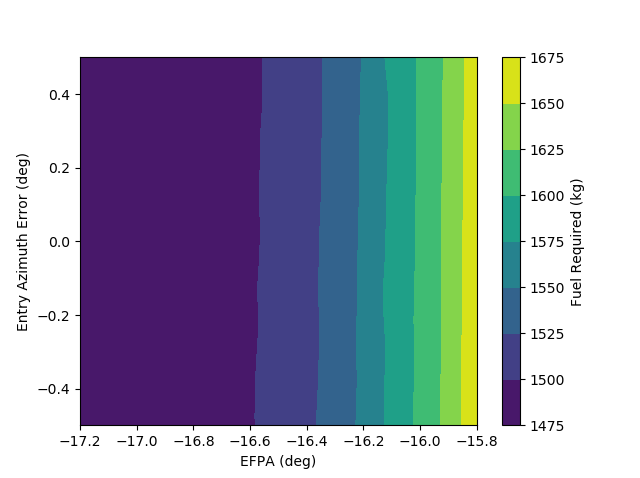
\includegraphics[width=1\textwidth]{optimal_fuel} 
%	\caption{Propellant required for different entry flight path angles and heading angles.}
%	\label{fig_sweep}
%\end{figure}

%\section{Conclusion}

\bibliographystyle{AAS_publication}
\bibliography{bib}

%\appendix
%\section{PMF Table Construction Procedure}
%Given a function $P(x)$ that produces an estimate of the propellant cost $m_{prop}$ to reach the target state from the current state $x$, we would like a procedure to effectively cover the set of points $X = \left\lbrace x\, |\, P(x) \le m_{\max} \right\rbrace $. 


\end{document}